% =====================================================================
% sections/02-mlops-concepts.tex  --  Member A
% Contains two sections:
%   \section{MLOps Concepts}            \label{sec:mlops-concepts}
%   \section{Overview of Michelangelo}  \label{sec:michelangelo-overview}
% Required packages in main.tex: booktabs, graphicx, amsmath (or amssymb)
% Figure: figures/michelangelo-workflow.pdf (fig:workflow)
% =====================================================================

\section{MLOps Concepts}
\label{sec:mlops-concepts}

Kreuzberger et al.\ define MLOps as a paradigm, comprising best practices,
concepts and a development culture, for the end-to-end conceptualisation,
implementation, monitoring, deployment and scalability of ML products; it
aims to productionise ML systems by bridging development and
operations~\cite{kreuzberger2023mlops}. Their study identifies nine
principles, including CI/CD automation, versioning, continuous training,
metadata tracking and continuous monitoring, which are realised by
technical components such as a feature store, a model registry and a
monitoring component~\cite{kreuzberger2023mlops}. This section introduces
the six concepts used throughout the report. For each concept we give a
definition from the literature and its counterpart in Michelangelo;
Table~\ref{tab:concept-mapping} summarises the mapping.

\subsection{ML Lifecycle}
\label{subsec:ml-lifecycle}

The \emph{ML lifecycle} is the sequence of activities required to build
and operate an ML model. Amershi et al.\ describe a nine-stage workflow
observed at Microsoft: model requirements, data collection, data
cleaning, data labelling, feature engineering, model training, model
evaluation, model deployment and model monitoring~\cite{amershi2019software}.
Unlike a conventional software process, this workflow is data-centric and
highly non-linear: evaluation and monitoring results frequently feed back
into earlier stages, for example when a distribution shift between
training and production data requires collecting new
data~\cite{amershi2019software}.
\textbf{In Michelangelo}, the lifecycle is condensed into a six-step
workflow (manage data, train, evaluate, deploy, predict, monitor) that
Uber reports to be shared by almost all of its ML use
cases~\cite{delbalso2017meet}. The platform is organised around this
workflow (Section~\ref{subsec:six-step-workflow}).

\subsection{CI/CD and Continuous Training}
\label{subsec:cicd-ct}

\emph{Continuous integration and continuous delivery/deployment} (CI/CD)
automate the build, test, delivery and deployment steps and give
developers rapid feedback~\cite{kreuzberger2023mlops}. ML adds a third
practice, \emph{continuous training} (CT): the periodic retraining of a
model on new feature data, enabled by a monitoring component, a feedback
loop and an automated workflow pipeline, and always accompanied by an
evaluation run that assesses the change in model
quality~\cite{kreuzberger2023mlops}.
\textbf{In Michelangelo}, early automation was exposed through an API:
many teams scheduled regular retraining and redeployment with their own
scripts, while others, such as the UberEATS delivery-time team, still
triggered both steps manually from the web UI~\cite{delbalso2017meet}.
Gallery added rule-based automation: user-defined rules over stored
performance metrics can detect model drift, raise alerts and trigger
retraining for an individual model, for example for a single city,
instead of retraining all models blindly~\cite{sun2020gallery}.
CI/CD became a platform capability with Project Canvas (2020), which
stores all ML code and configuration in a monorepo, packages training
and serving code into immutable Docker images, and automatically deploys
models merged into the main branch after tests and
validations~\cite{wang2024predictive}. The unified MA Studio interface
adds incremental zonal rollout with automatic rollback triggers to
deployment~\cite{wang2024predictive}.

\subsection{Feature Store}
\label{subsec:feature-store}

A \emph{feature store} provides central storage for commonly used
features and typically combines an offline store, which serves features
with normal latency for experimentation and training, with an online
store, which serves features with low latency for production
inference~\cite{kreuzberger2023mlops}. Feature stores emerged to avoid
duplicated feature engineering across teams and inconsistent feature
definitions, and to keep deployed models supplied with fresh
features~\cite{orr2021managing}.
\textbf{In Michelangelo}, the feature store (later named
\emph{Palette}) uses Hive as the offline store and Cassandra as the
online store; features are computed by Spark batch jobs or by Samza
streaming jobs~\cite{li2017scaling}. A model refers to a feature only by
its canonical name, and the platform resolves the name to the correct
offline or online source~\cite{delbalso2017meet}. Uber reports freshness
guarantees of under 12 hours for historical features and under 5 minutes
for near-real-time features, each served with about 10\,ms query
latency~\cite{li2017scaling}. The store grew from approximately 10{,}000
features in 2017~\cite{delbalso2017meet} to more than 20{,}000 in
2024~\cite{wang2024predictive}.

\subsection{Model Registry}
\label{subsec:model-registry}

A \emph{model registry} centrally stores trained models together with
their metadata, such as training parameters, performance metrics and
lineage, to support reproducibility and versioning~\cite{kreuzberger2023mlops}.
Open-source platforms such as MLflow address the same need for tracking
experiments and packaging models for deployment~\cite{zaharia2018accelerating}.
\textbf{In Michelangelo}, every trained model is stored as a versioned
object that records, among other things, who trained it, its full
configuration, references to the training and test data, feature
importance, accuracy metrics and the learned
parameters~\cite{delbalso2017meet}. At serving time, a client addresses a
model either by its UUID or by a tag; deploying a new model with the same
signature to an existing tag switches traffic to it without any change to
client code~\cite{delbalso2017meet}.

The registry role was later consolidated in \emph{Gallery}, a model
lifecycle management system originally built by Uber's Marketplace
Forecasting team and subsequently integrated into
Michelangelo~\cite{sun2020gallery}. Before Gallery, Uber engineers used
more than seven different storage solutions to save models, including
MySQL, HDFS, Cassandra and Git repositories~\cite{sun2020gallery}. Gallery
is designed around four principles: models are \emph{immutable}, so every
update creates a new version; the system is \emph{model-neutral} and
\emph{framework-agnostic}, storing trained models as uninterpreted binary
blobs; and lifecycle transitions are \emph{automated}~\cite{sun2020gallery}.
It distinguishes a \emph{model} (the specification of a transformation,
such as features and hyper-parameters) from a \emph{model instance} (the
parameters learned from a particular training set), assigns each instance
a Git-style UUID linked to a base version, and tracks dependencies
between models whose outputs feed one another~\cite{sun2020gallery}.
Metadata and metrics are kept in a relational database for search, while
model blobs reside in distributed storage~\cite{sun2020gallery}. A rule
engine evaluates user-defined, peer-reviewed rules over these metrics,
either to select a \emph{champion} model for serving or to trigger actions
such as deployment~\cite{sun2020gallery}. As part of Michelangelo, Gallery
manages more than one million model instances, and for Uber's forecasting
models it reduced deployment effort from two hours of engineering work
per model to none~\cite{sun2020gallery}. Our demonstrator reproduces the
tag-based switching mechanism with MLflow model aliases.

\subsection{Training/Serving Skew}
\label{subsec:train-serve-skew}

\emph{Training/serving skew} is a discrepancy between the data used to
train a model and the data it receives in production. Breck et al.\
identify the use of different code paths to generate training and
serving data as its most common cause, and distinguish three forms:
\emph{feature skew} (a feature takes different values at training and
serving time), \emph{distribution skew} (the feature distribution in
training differs from that at serving time) and \emph{scoring/serving
skew} (only a subset of scored examples is actually served, which biases
future training data)~\cite{breck2019data}.
\textbf{In Michelangelo}, the primary safeguard is a single code path:
each feature is computed by one pipeline for both training and
prediction~\cite{li2017scaling}, and feature selection and transformation
are expressed in a domain-specific language (DSL) whose expressions are
stored in the model configuration and applied identically at training
and prediction time~\cite{delbalso2017meet}. In Michelangelo~2.0, the
transformations are bundled with the model, including DL-native
transformations compiled into the inference graph, and MA Studio provides
an online/offline feature consistency check~\cite{wang2024predictive}.
At the model level, Gallery stores training, validation and production
metrics for every model instance, so that \emph{production skew}, a gap
between training-time and serving-time performance, can be
detected~\cite{sun2020gallery}.

\subsection{Monitoring and Drift}
\label{subsec:monitoring-drift}

Because the external world is rarely stable, live monitoring combined
with automated response is critical for the long-term reliability of ML
systems~\cite{sculley2015hidden}. A principal reason is \emph{concept
drift}, formally a change in the joint distribution of inputs $X$ and
target $y$ between two points in time~\cite{gama2014survey}:
\begin{equation}
  \exists X : p_{t_0}(X, y) \neq p_{t_1}(X, y).
  \label{eq:concept-drift}
\end{equation}
Gama et al.\ distinguish \emph{real} concept drift, a change in
$p(y \mid X)$ that affects predictive decisions, from \emph{virtual}
drift, a change in the input distribution $p(X)$ that does not affect
$p(y \mid X)$~\cite{gama2014survey}. Continuous monitoring therefore
covers data, model and serving performance~\cite{kreuzberger2023mlops}.
\textbf{In Michelangelo}, two complementary approaches are used. When
outcomes are observable, the platform logs predictions, joins them with
the observed labels and publishes accuracy metrics (e.g., RMSE and MAE)
to Uber's time-series monitoring system with threshold
alerts~\cite{delbalso2017meet,li2017scaling}. When labels are delayed or
unavailable, it compares the distributions of features and predictions
over time, which is less precise but still detects problematic
shifts~\cite{delbalso2018scaling}. Since Michelangelo~2.0, a Model
Excellence Score (MES) tracks quality dimensions such as prediction
accuracy, model freshness and feature quality against SLA-style
targets~\cite{wang2024predictive}.

\begin{table}[t]
  \centering
  \caption{MLOps concepts and their realisation in Michelangelo.}
  \label{tab:concept-mapping}
  \small
  \begin{tabular}{@{}p{0.22\linewidth}p{0.72\linewidth}@{}}
    \toprule
    \textbf{Concept} & \textbf{Michelangelo realisation} \\
    \midrule
    ML lifecycle &
      Six-step workflow shared by most use cases~\cite{delbalso2017meet} \\
    CI/CD/CT &
      API-scheduled retraining~\cite{delbalso2017meet}; rule-triggered
      retraining in Gallery~\cite{sun2020gallery}; Canvas monorepo, ML CI/CD
      and immutable images~\cite{wang2024predictive} \\
    Feature store &
      Palette: Hive (offline) and Cassandra (online), canonical feature
      names~\cite{li2017scaling,delbalso2017meet} \\
    Model registry &
      Versioned model repository with UUID/tag addressing~\cite{delbalso2017meet};
      Gallery: immutable model instances, metadata search, rule-based
      champion selection~\cite{sun2020gallery} \\
    Training/serving skew &
      One feature code path; shared DSL; consistency
      check~\cite{li2017scaling,delbalso2017meet,wang2024predictive} \\
    Monitoring \& drift &
      Prediction--outcome joins; distribution monitoring;
      MES~\cite{delbalso2017meet,delbalso2018scaling,wang2024predictive} \\
    \bottomrule
  \end{tabular}
\end{table}

% ---------------------------------------------------------------------

\section{Overview of Michelangelo}
\label{sec:michelangelo-overview}

\subsection{Evolution from 2015 to 2024}
\label{subsec:evolution}

Uber began building Michelangelo in mid-2015~\cite{delbalso2017meet}, and
dates the first production version to 2016~\cite{wang2024predictive}.
Table~\ref{tab:timeline} summarises the three phases identified by
Uber~\cite{wang2024predictive}, each with representative metrics.

\emph{Michelangelo~1.0 (2016--2019)} targeted predictive ML on tabular
data, using algorithms such as XGBoost for ETA prediction, risk
assessment and pricing~\cite{wang2024predictive}. The initial focus was
large-scale batch training and batch prediction; a centralised feature
store, a low-latency real-time prediction service, DL workflows,
notebook integration and partitioned models were added
incrementally~\cite{delbalso2018scaling}.

\emph{Michelangelo~2.0 (2019--2023)} shifted the focus from enabling ML
everywhere to improving high-impact projects. It addressed four
shortcomings of version~1.0: the lack of a model-quality definition and
project tiering, insufficient DL support, poor support for collaborative
development, and fragmented tooling~\cite{wang2024predictive}. The
response included project tiering, model iteration as code via Canvas,
DL as a first-class citizen (Ray-based trainers and Triton-based
serving), and the unified MA Studio interface~\cite{wang2024predictive}.
Architecturally, the platform was reorganised into a control plane, an
offline data plane and an online data plane~\cite{wang2024predictive};
this structure is analysed in Section~\ref{sec:layered-architecture}.

\emph{Generative AI (2023--present)} extended the platform to LLMOps. A
Gen AI Gateway provides unified, policy-controlled access to external
and in-house large language models (LLMs), and the platform added a model
catalogue, an LLM evaluation framework, a prompt engineering toolkit, and
fine-tuning based on Hugging Face and DeepSpeed~\cite{wang2024predictive}.

\begin{table}[t]
  \centering
  \caption{Evolution of Michelangelo (phases as defined by Uber~\cite{wang2024predictive}).}
  \label{tab:timeline}
  \small
  \begin{tabular}{@{}p{0.17\linewidth}p{0.36\linewidth}p{0.39\linewidth}@{}}
    \toprule
    \textbf{Phase} & \textbf{Focus and key additions} & \textbf{Representative metrics} \\
    \midrule
    1.0 \newline (2016--2019) &
      Predictive ML on tabular data; feature store; real-time serving;
      partitioned models; Gallery; PyML; Horovod~\cite{delbalso2018scaling,wang2024predictive} &
      2017: $\approx$10{,}000 features; online P95 latency $<$10\,ms; top
      models $>$250{,}000 predictions/s~\cite{delbalso2017meet}.
      2018: thousands of production models; millions of predictions/s~\cite{delbalso2018scaling} \\
    \addlinespace
    2.0 \newline (2019--2023) &
      DL as first-class citizen; Canvas (2020); MA Studio; project
      tiering; Ray and Triton; three-plane architecture~\cite{wang2024predictive} &
      2020: $>$1\,M model instances managed by Gallery~\cite{sun2020gallery}.
      $>$5{,}000 GPUs; DL adoption in tier-1 projects from almost zero to
      $>$60\,\%~\cite{wang2024predictive} \\
    \addlinespace
    GenAI \newline (2023--) &
      Gen AI Gateway; LLM fine-tuning, evaluation and prompt
      management~\cite{wang2024predictive} &
      2024: $\approx$400 active projects; $>$20{,}000 training jobs/month;
      $>$5{,}000 production models; 10\,M predictions/s at peak~\cite{wang2024predictive} \\
    \bottomrule
  \end{tabular}
\end{table}

\subsection{The Six-Step Workflow}
\label{subsec:six-step-workflow}

Michelangelo was designed to provide scalable, reliable, reproducible
and automated tooling for a six-step workflow~\cite{delbalso2017meet},
illustrated in Figure~\ref{fig:workflow} and summarised below using
UberEATS estimated time of delivery (ETD) as the running example. The
ETD model is a gradient-boosted decision tree regressor whose features
combine request data, historical aggregates and near-real-time
aggregates~\cite{delbalso2017meet}.

\begin{enumerate}
  \item \textbf{Manage data.} Offline pipelines compute features from
    the HDFS data lake with Spark and Hive; online features are
    precomputed into Cassandra either by batch jobs or by Samza streaming
    jobs consuming Kafka~\cite{delbalso2017meet}. For ETD, a restaurant's
    average meal preparation time over the last seven days is a batch
    feature, whereas the same average over the last hour is a
    near-real-time feature~\cite{delbalso2017meet}.
  \item \textbf{Train models.} A model configuration specifies the
    model type, hyper-parameters, data source, feature DSL expressions
    and compute resources, and training runs as a distributed
    job~\cite{delbalso2017meet}. \emph{Partitioned models} train one model
    per node of a hierarchy (e.g., city and country) and fall back to the
    parent model when a partition lacks data; ETD is trained in this way
    as a single logical model for all cities~\cite{li2017scaling}.
  \item \textbf{Evaluate models.} Each trained model is stored in the
    model repository with accuracy reports, feature-importance reports and
    visualisations, enabling comparison across many candidate
    models~\cite{delbalso2017meet}.
  \item \textbf{Deploy models.} Models can be deployed offline (batch
    prediction in Spark jobs), online (a prediction service cluster
    called via RPC), or as an embedded library; model artifacts are
    distributed through Uber's standard code deployment
    infrastructure~\cite{delbalso2017meet}.
  \item \textbf{Make predictions.} The serving container applies the
    compiled DSL to raw features, fetches additional features from the
    feature store, and scores the final feature
    vector~\cite{delbalso2017meet}. Uber reports a 99th-percentile latency
    of 20\,ms for ETD serving under bursty meal-time
    traffic~\cite{li2017scaling}.
  \item \textbf{Monitor predictions.} Predictions are logged and joined
    with observed outcomes to compute live accuracy metrics and trigger
    alerts (Section~\ref{subsec:monitoring-drift}).
\end{enumerate}

\begin{figure}[t]
  \centering
  % Source files: figures/michelangelo-workflow.tex (TikZ),
  %               figures/michelangelo-workflow.drawio (editable copy for F).
  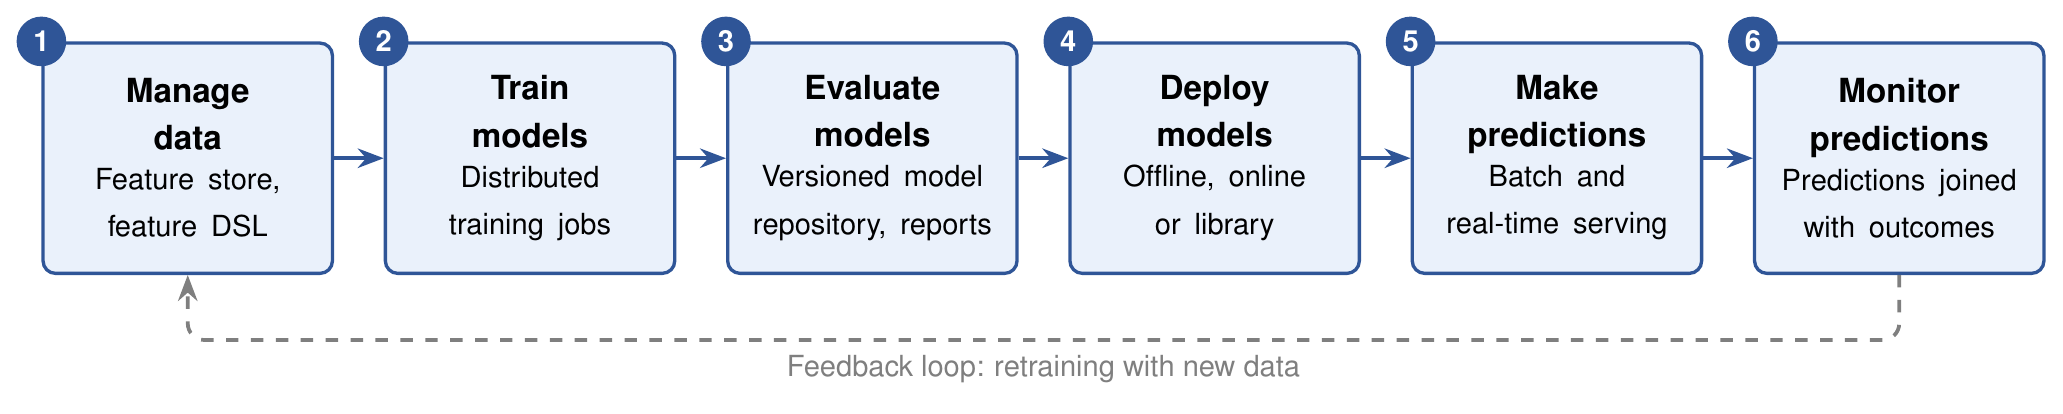
\includegraphics[width=\linewidth]{figures/michelangelo-workflow}
  \caption{Michelangelo's six-step ML workflow, based
    on~\cite{delbalso2017meet}. The dashed arrow denotes the feedback loop
    from monitoring back to data management and retraining.}
  \label{fig:workflow}
\end{figure}

A management plane, comprising a web UI, a REST API and a workflow
system, orchestrates data pipelines, training jobs, batch prediction and
model deployment across these steps~\cite{delbalso2017meet}. How this
plane and the data-processing components are layered, and how that
layering changed in Michelangelo~2.0, is the subject of
Section~\ref{sec:layered-architecture}.